\def\recbase{5}
\def\recheight{1}

\begin{figure}

\begin{center}
  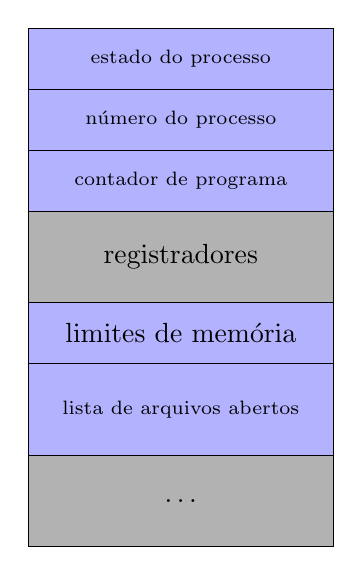
\begin{tikzpicture}[every rectangle/.style={minimum width=\recbase},
    scale=0.775,mem/.style={fill=gray!60},
    var/.style={fill=blue!30}]
    
    \draw[var] (0,2+5.5*\recheight) rectangle (\recbase,2+6.5*\recheight)
    node[midway] {\scriptsize{estado do processo}};
    \draw[var] (0,2+4.5*\recheight) rectangle (\recbase,2+5.5*\recheight)
    node[midway] {\scriptsize{número do processo}};
    \draw[var] (0,2+3.5*\recheight) rectangle (\recbase,2+4.5*\recheight)
    node[midway] {\scriptsize{contador de programa}};
    \draw[mem] (0,2+2*\recheight) rectangle (\recbase,2+3.5*\recheight) node[midway] {registradores};
    \draw[var] (0,2+\recheight) rectangle (\recbase,2+2*\recheight) node[midway] {limites de
    memória};
    \draw[var] (0,1.5) rectangle (\recbase,2+\recheight) node[midway] {\scriptsize{lista de
    arquivos abertos}};
    \draw[mem] (0,0) rectangle (\recbase,1.5*\recheight) node[midway] {$\ldots$};
  \end{tikzpicture}
\end{center}

\caption{Bloco de controle do processo.}
\label{proc:fig:pcb}

\end{figure}
